\documentclass{homework}

\title{Problem Set 2}
\author{Kevin Evans}
\studentid{11571810}
\date{February 9, 2021}
\setclass{Physics}{463}
\usepackage{amssymb}
\usepackage{mathtools}
\usepackage{graphicx}
\usepackage{amsthm}
\usepackage{amsmath}
\usepackage{slashed}
\usepackage{boldline}
\usepackage{physics}
\usepackage{tcolorbox}
\usepackage[inter-unit-product =\cdot]{siunitx}

\usepackage[makeroom]{cancel}
\usepackage{booktabs}
\usepackage{multirow}

\usepackage{times}
\usepackage{mhchem}
\usepackage{enumitem}
\usepackage[normalem]{ulem}
\usepackage{systeme}
\usepackage{tikz}
\usepackage{mathtools}
\usepackage{tabularx}
\usepackage{listings}
\usepackage{breqn}


\newcommand{\fm}{\femto\meter}


\begin{document}
	\maketitle
	\begin{enumerate}
		\item % 2.1
			\begin{enumerate}
				\item Following what we did in-class, for a plane $(hkl)$ and reciprocal lattice vector $$\bvec{G} = h \bvec{b}_1 + k \bvec{b}_2 + l \bvec{b}_3,$$
				if we consider a plane on $hkl$ defined by two noncolinear vectors \begin{align*}
					\bvec{A} & = \frac{1}{h} \bvec{a}_1 - \frac{1}{l} \bvec{a}_3 \\
					\bvec{B} & = -\frac{1}{h} \bvec{a}_1 + \frac{1}{k} \bvec{a}_2,
					\intertext{we are to show that}
					\bvec{G} \cdot \bvec{A}&  = \bvec{G} \cdot \bvec{B} = 0 \iff \bvec{G} \perp (hkl).
				\end{align*}
				Using $\bvec{b}_i \cdot \bvec{a}_j = 2 \pi \delta_{ij}$, \begin{align*}
					\bvec{G} \cdot \bvec{A} & = 2 \pi h / h - 2 \pi l / l = 0, \\
					\bvec{G} \cdot \bvec{B} & = -2 \pi h / h + 2 \pi l / l = 0.  \qed\\
				\end{align*}
			
				\item The distance from the origin to the plane $\bvec{G}$ is \begin{align*}
					d(hkl) & = \frac{1}{h} \bvec{a}_1 \cdot \uvec{n} = \frac{1}{h} \bvec{a}_1 \cdot \bvec{G} / \abs{G} \\
						& = \frac{1}{G} (2 \pi h / h) = 2 \pi / G. \qed
				\end{align*}
			
				\item For an sc lattice of separation $a$, we can define $\bvec{G}$ as \begin{align*}
					\bvec{G} & = 2 \pi / a \left(h\uvec{x} + k\uvec{y} l\uvec{z}\right).
					\intertext{Then, the squared distance from the origin to the plane is }
					d^2 & = (2 \pi)^2 / G^2 \\
						& = a^2 / (h^2 + k^2 + l^2). \qed
				\end{align*}
			\end{enumerate}
		\item % 2.2
			\begin{enumerate}
				\item The volume of a primitive cell is defined $$V = \bvec{a}_1 \cdot (\bvec{a}_2 \cross \bvec{a}_3).$$
					
					For this hexagonal space lattice, \begin{align*}
						V_c & = \bvec{a}_1 \cdot \left[
							\left( -3^{1/2} a/2 \uvec{x} + a/2 \uvec{y} \right)
							\cross c \uvec{z}
						\right] \\
							& = \bvec{a}_1 \cdot \left[
								3^{1/2} ac/2 \uvec{y}
								+ ac/2 \uvec{x}
							\right] \\
							& = \left(3^{1/2} a/2 \uvec{x} + a/2 \uvec{y}\right)\cdot \left(
							3^{1/2} ac/2 \uvec{y}
							+ ac/2 \uvec{x}
							\right) \\
							& = 2 \times 3^{1/2}a^2/4 c \\
							& = (3^{1/2}/2) a^2 c. \qed
					\end{align*}
				
				\item The reciprocal lattice's primitive translation vectors are \begin{align*}
						\bvec{b}_1 & \equiv 2 \pi \frac{\bvec{a}_2 \cross \bvec{a}_3}{V_c} \\
							& = \frac{2 \pi}{V_c} \left[
								\left(-(3^{1/2}a/2) \uvec{x} + (a/2)\uvec{y}\right)
								\cross
								\left(c\uvec{z}\right)
							\right] \\
							& = \frac{2 \pi}{V_c} \left[
								(3^{1/2} ac/2) \uvec{y}
								+ (ac/2) \uvec{x}
							\right]
						\intertext{Substituting the primitive cell from part (b),}
						\bvec{b}_1 & = (2 \pi / 3^{1/2} a) \uvec{x} + (2 \pi / a) \uvec{y}. \qed
						\intertext{For the next vector,}
						\bvec{b}_2 & \equiv \frac{2 \pi}{V_c} \bvec{a}_3 \cross \bvec{a}_1 \\
							& = \frac{2 \pi}{V_c}\left\{
								c \uvec{z}
								\cross
								\left[
									(3^{1/2} a/2) \uvec{x}
									+
									(a/2) \uvec{y}
								\right]
							\right\} \\
							& = \frac{2 \pi}{V_c} \left\{
								(3^{1/2} ac/2) \uvec{y}
								- (ac/2) \uvec{x}
							\right\} \\
							& = -(2 \pi / 3^{1/2}a) \uvec{x} + (2 \pi / a) \uvec{y}. \qed
							\intertext{Lastly,}
							\bvec{b}_3 & \equiv \frac{2 \pi}{V_c} \bvec{a}_1 \cross \bvec{a}_2 \\
								& = \frac{2 \pi}{V_c} \left\{
									\left[
										(3^{1/2} a / 2)\uvec{x} 
										+
										(a/2) \uvec{y}
									\right]
									\cross
									\left[
										-(3^{1/2} a / 2) \uvec{x}
										+
										(a/2) \uvec{y}
									\right]
								\right\}
							\intertext{Since only the cross term is non-zero, this reduces to}
							\bvec{b}_3 & = \frac{2 \pi}{V_c} \left\{
									2 \times (3^{1/2} a^2 / 4) \uvec{z}
								\right\} \\
									& = (2 \pi / c) \uvec{z}. \qed
					\end{align*}
				
				\item The reciprocal lattice is also hexagonal, as it follows roughly the same vectors of the initial lattice. We can begin by finding the neighboring reciprocal lattice points,
				
				It'd probably roughly look something like this: \begin{center}
					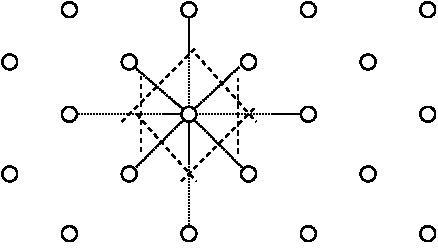
\includegraphics{hex.pdf}
				\end{center}
				
			\end{enumerate}
		
		\item % 2.3
			The volume of the FBZ is given by \begin{align*}
				V = \bvec{b}_1 \cdot \left(\bvec{b}_2 \cross \bvec{b}_3\right) & = \frac{(2 \pi)^3}{(V_c)^3} \left(
					\left(\bvec{a}_2 \cross \bvec{a_3}\right) \cdot \left[
						\left(\bvec{a}_3 \cross \bvec{a}_1\right) \cross 
						\left(\bvec{a}_1 \cross \bvec{a}_2\right)
					\right]
				\right)
				\intertext{Using the hint of $(c\cross a) \cross (a \cross b) = (c \cdot a \cross b) a$,}
				V & = \frac{(2 \pi)^3}{(V_c)^3} \left\{
					(\bvec{a}_2 \cross \bvec{a}_3) \cdot \left[
						\bvec{a}_3 \cdot \bvec{a}_1 \cross \bvec{a}_2
					\right] \bvec{a}_1
				\right\} \\
					& = \frac{(2 \pi)^3}{(V_c)^3} \left\{
						(\bvec{a}_2 \cross \bvec{a}_3) \cdot
						\left[
							\bvec{a}_1 \cdot \bvec{a}_2 \cross \bvec{a}_3
						\right] \bvec{a}_1
					\right\} && \text{triple prod.}\\
					& = \frac{(2 \pi)^3}{(V_c)^3} \left\{
						\underbrace{\bvec{a}_1 \cdot ( \bvec{a}_2 \cross \bvec{a}_3)}_{V_c} V_c
					\right\} \\
					& = \frac{(2 \pi)^3}{(V_c)^2} {V_c}^3 = (2 \pi)^3 / V_c. \qed
			\end{align*}
		
		\pagebreak
		
		\item % 2.5
			\begin{enumerate}
				\item The structure factor is given by an fcc lattice with atoms at two points, $(0, 0, 0)$, and $(1/4, 1/4, 1/4)$. We can use equation (48) for the fcc structure factor at $(0, 0, 0)$, then tack on the additional points at $(1/4, 1/4, 1/4)$. These additional points will be the regular fcc lattice points, offset by $(1/4, 1/4, 1/4)$, 
				$$\{(1/4, 1/4, 1/4), (3/4, 3/4, 1/4),  (1/4, 3/4, 3/4), (3/4, 1/4, 3/4)\}.$$
				The additional terms in the structure factor are
				\begin{align*}
					S_{1/4} & = f \Big\{
						\exp[-i2 \pi (v_1 + v_2 + v_3)/4] + \exp[-i2 \pi(3v_1 + 3v_2 + v_3)/4] \\
						& \qquad + \exp[-i2\pi(v_1 + 3 v_2 + 3 v_3) / 4] + \exp[-i2 \pi (3 v_1 + v_2 + 3v_3) / 4]\Big\}.
				\end{align*}
				Combining this with the original fcc structure factor,
				 \begin{align*}
					S(v_1 v_2 v_3) & = f \Big\{
						1 + \exp[-i \pi (v_2 + v_3)]+ \exp[-i \pi (v_1 + v_3)] + \exp[-i \pi (v_1 + v_2)] \\
						& \hspace{3em} + \exp[-i \pi (v_1 + v_2 + v_3)/2] + \exp[-i \pi(3v_1 + 3v_2 + v_3)/2] \\
						& \hspace{3em} + \exp[-i\pi(v_1 + 3 v_2 + 3 v_3) / 2] + \exp[-i \pi (3 v_1 + v_2 + 3v_3) / 2]\Big\}.
				\end{align*}
				
				
				\item  I'm not sure of the best way to do this analytically, so I wrote a short Python script to do this\footnote{Attached at end.}. Since the complex exponential is repeating for $v_i \mod 4$, we can just iterate over $0$ to $3$ for each variable. This resulted in \begin{align*}
					S & = \begin{cases*}
						0 & 2 indices odd, 1 even \\
						0 & 1 index odd, 2 even \\
						8f & all even and all sum to 4
					\end{cases*}
				\end{align*}
			\end{enumerate}
		
		\pagebreak
		
		\item In this problem, I'm just going to ignore the other two directions needed to find a reciprocal lattice. It's implied the direct lattice spacing in those directions is infinite and the reciprocal lattice spacing is then zero.
		 \begin{enumerate}
			\item For a one-dimensional crystal with spacing $d$, then the reciprocal translation vector will be $$b_1 = 2 \pi / d.$$ The first Brillouin zone will be a line segment of $2\pi/d$ length,
			\begin{center}
				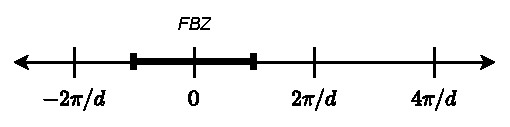
\includegraphics{fbz.pdf}
			\end{center}
			
			\item If they're alternating, then the direct lattice has a side length of $2d$. Then the FBZ will be a line segment of $\pi/d$,
			\begin{center}
				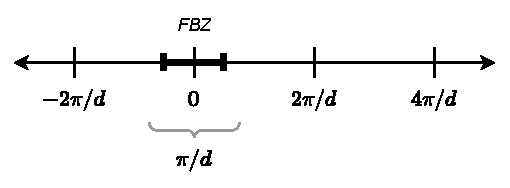
\includegraphics{fbz2.pdf}
			\end{center}
		\end{enumerate}
	\end{enumerate}

	\pagebreak
	\begin{lstlisting}[language=python,title={Python code to determine $v_1, v_2, v_3 \mod 4$ values which produce zeros and maxima.}]
import numpy as np

i = 1j
pi = np.pi
exp = np.exp

for x in range(0, 4):
	for y in range(0, 4):
		for z in range(0, 4):
			S = 1 + exp(-i*pi*(y+z)) + exp(-i*pi*(x+z)) + exp(-i*pi*(x+y)) \ 
				+ exp(-i*pi*(x+y+z)/2) + exp(-i*pi*(3*x + 3*y+z)/2) \
				+ exp(-i*pi*(x+3*y+3*z)/2) + exp(-i*pi*(3*x+y+3*z)/2)
			print(f"{x}\t{y}\t{z}\t{np.around(S, decimals=9) or '0' }")
	\end{lstlisting}

	\begin{lstlisting}[title={Python code output.}]
0	0	0	(8+0j)
0	0	1	0
0	0	2	0
0	0	3	0
0	1	0	0
0	1	1	0
0	1	2	0
0	1	3	0
0	2	0	0
0	2	1	0
0	2	2	(8+0j)
0	2	3	0
0	3	0	0
0	3	1	0
0	3	2	0
0	3	3	0
1	0	0	0
1	0	1	0
1	0	2	0
1	0	3	0
1	1	0	0
1	1	1	(4+4j)
1	1	2	0
1	1	3	(4-4j)
1	2	0	0
1	2	1	0
1	2	2	0
1	2	3	0
1	3	0	0
1	3	1	(4-4j)
1	3	2	0
1	3	3	(4+4j)
2	0	0	0
2	0	1	0
2	0	2	(8+0j)
2	0	3	0
2	1	0	0
2	1	1	0
2	1	2	0
2	1	3	0
2	2	0	(8+0j)
2	2	1	0
2	2	2	0
2	2	3	0
2	3	0	0
2	3	1	0
2	3	2	0
2	3	3	0
3	0	0	0
3	0	1	0
3	0	2	0
3	0	3	0
3	1	0	0
3	1	1	(4-4j)
3	1	2	0
3	1	3	(4+4j)
3	2	0	0
3	2	1	0
3	2	2	0
3	2	3	0
3	3	0	0
3	3	1	(4+4j)
3	3	2	0
3	3	3	(4-4j)
\end{lstlisting}
\end{document}
		